\documentclass[12pt,a4paper,]{article}
\usepackage{booktabs}
\usepackage{rotating}
\usepackage{lmodern}
\usepackage{amssymb,amsmath}
\usepackage{ifxetex,ifluatex}
\usepackage{fixltx2e} % provides \textsubscript
\ifnum 0\ifxetex 1\fi\ifluatex 1\fi=0 % if pdftex
  \usepackage[T1]{fontenc}
  \usepackage[utf8x]{inputenc}
\else % if luatex or xelatex
  \ifxetex
    \usepackage{mathspec}
  \else
    \usepackage{fontspec}
  \fi
  \defaultfontfeatures{Ligatures=TeX,Scale=MatchLowercase}
\fi
% use upquote if available, for straight quotes in verbatim environments
\IfFileExists{upquote.sty}{\usepackage{upquote}}{}
% use microtype if available
\IfFileExists{microtype.sty}{%
\usepackage{microtype}
\UseMicrotypeSet[protrusion]{basicmath} % disable protrusion for tt fonts
}{}
\usepackage{hyperref}
\hypersetup{unicode=true,
            pdfborder={0 0 0},
            breaklinks=true}
\urlstyle{same}  % don't use monospace font for urls
\usepackage{color}
\usepackage{fancyvrb}
\newcommand{\VerbBar}{|}
\newcommand{\VERB}{\Verb[commandchars=\\\{\}]}
\DefineVerbatimEnvironment{Highlighting}{Verbatim}{commandchars=\\\{\}}
% Add ',fontsize=\small' for more characters per line
\newenvironment{Shaded}{\footnotesize}{}
\newcommand{\KeywordTok}[1]{\textcolor[rgb]{0.00,0.44,0.13}{\textbf{{#1}}}}
\newcommand{\DataTypeTok}[1]{\textcolor[rgb]{0.56,0.13,0.00}{{#1}}}
\newcommand{\DecValTok}[1]{\textcolor[rgb]{0.25,0.63,0.44}{{#1}}}
\newcommand{\BaseNTok}[1]{\textcolor[rgb]{0.25,0.63,0.44}{{#1}}}
\newcommand{\FloatTok}[1]{\textcolor[rgb]{0.25,0.63,0.44}{{#1}}}
\newcommand{\ConstantTok}[1]{\textcolor[rgb]{0.53,0.00,0.00}{{#1}}}
\newcommand{\CharTok}[1]{\textcolor[rgb]{0.25,0.44,0.63}{{#1}}}
\newcommand{\SpecialCharTok}[1]{\textcolor[rgb]{0.25,0.44,0.63}{{#1}}}
\newcommand{\StringTok}[1]{\textcolor[rgb]{0.25,0.44,0.63}{{#1}}}
\newcommand{\VerbatimStringTok}[1]{\textcolor[rgb]{0.25,0.44,0.63}{{#1}}}
\newcommand{\SpecialStringTok}[1]{\textcolor[rgb]{0.73,0.40,0.53}{{#1}}}
\newcommand{\ImportTok}[1]{{#1}}
\newcommand{\CommentTok}[1]{\textcolor[rgb]{0.38,0.63,0.69}{\textit{{#1}}}}
\newcommand{\DocumentationTok}[1]{\textcolor[rgb]{0.73,0.13,0.13}{\textit{{#1}}}}
\newcommand{\AnnotationTok}[1]{\textcolor[rgb]{0.38,0.63,0.69}{\textbf{\textit{{#1}}}}}
\newcommand{\CommentVarTok}[1]{\textcolor[rgb]{0.38,0.63,0.69}{\textbf{\textit{{#1}}}}}
\newcommand{\OtherTok}[1]{\textcolor[rgb]{0.00,0.44,0.13}{{#1}}}
\newcommand{\FunctionTok}[1]{\textcolor[rgb]{0.02,0.16,0.49}{{#1}}}
\newcommand{\VariableTok}[1]{\textcolor[rgb]{0.10,0.09,0.49}{{#1}}}
\newcommand{\ControlFlowTok}[1]{\textcolor[rgb]{0.00,0.44,0.13}{\textbf{{#1}}}}
\newcommand{\OperatorTok}[1]{\textcolor[rgb]{0.40,0.40,0.40}{{#1}}}
\newcommand{\BuiltInTok}[1]{{#1}}
\newcommand{\ExtensionTok}[1]{{#1}}
\newcommand{\PreprocessorTok}[1]{\textcolor[rgb]{0.74,0.48,0.00}{{#1}}}
\newcommand{\AttributeTok}[1]{\textcolor[rgb]{0.49,0.56,0.16}{{#1}}}
\newcommand{\RegionMarkerTok}[1]{{#1}}
\newcommand{\InformationTok}[1]{\textcolor[rgb]{0.38,0.63,0.69}{\textbf{\textit{{#1}}}}}
\newcommand{\WarningTok}[1]{\textcolor[rgb]{0.38,0.63,0.69}{\textbf{\textit{{#1}}}}}
\newcommand{\AlertTok}[1]{\textcolor[rgb]{1.00,0.00,0.00}{\textbf{{#1}}}}
\newcommand{\ErrorTok}[1]{\textcolor[rgb]{1.00,0.00,0.00}{\textbf{{#1}}}}
\newcommand{\NormalTok}[1]{{#1}}
\usepackage{longtable,booktabs}
\usepackage{graphicx,grffile}
\makeatletter
\def\maxwidth{\ifdim\Gin@nat@width>\linewidth\linewidth\else\Gin@nat@width\fi}
\def\maxheight{\ifdim\Gin@nat@height>\textheight\textheight\else\Gin@nat@height\fi}
\makeatother
% Scale images if necessary, so that they will not overflow the page
% margins by default, and it is still possible to overwrite the defaults
% using explicit options in \includegraphics[width, height, ...]{}
\setkeys{Gin}{width=\maxwidth,height=\maxheight,keepaspectratio}
% Make links footnotes instead of hotlinks:
\renewcommand{\href}[2]{#2\footnote{See \texttt{\url{#1}}}}
\setlength{\emergencystretch}{3em}  % prevent overfull lines
\providecommand{\tightlist}{%
  \setlength{\itemsep}{0pt}\setlength{\parskip}{0pt}}
\setcounter{secnumdepth}{5}
% Redefines (sub)paragraphs to behave more like sections
\ifx\paragraph\undefined\else
\let\oldparagraph\paragraph
\renewcommand{\paragraph}[1]{\oldparagraph{#1}\mbox{}}
\fi
\ifx\subparagraph\undefined\else
\let\oldsubparagraph\subparagraph
\renewcommand{\subparagraph}[1]{\oldsubparagraph{#1}\mbox{}}
\fi

\date{}


%
% Line Spread, Page Markings & Hyperlinked Documents
%
\linespread{1.3}
% Margin:
\usepackage[top=1.5in, bottom=1.5in, right=1in, left=1in]{geometry}

% To silence too small headheight warning
\setlength{\headheight}{15pt}

% Header & Footer:
\usepackage{fancyhdr}
\pagestyle{fancy}
\fancyhf{} % Clear all header and footer fields
\fancyhead[LO,RE]{Helpdesk Ticketing System\\{\vspace{-2pt}\scriptsize Semester 1}}
\fancyhead[LE,RO]{\leftmark\\{\vspace{-4pt}\scriptsize SWE40001 Software Engineering Project}}
\fancyfoot[LE,RO]{\thepage\ifodd\value{page}\else\hfill\fi}
\usepackage{float}

\begin{document}

{
\setcounter{tocdepth}{3}
\tableofcontents
}
\newpage
\section{Doubtfire Git Workflow}\label{doubtfire-git-workflow}

We follow a
\href{https://www.atlassian.com/git/tutorials/comparing-workflows/forking-workflow}{Forking
workflow} when developing Doubtfire.

\subsection{Table of Contents}\label{table-of-contents}

\begin{enumerate}
\def\labelenumi{\arabic{enumi}.}
\tightlist
\item
  \protect\hyperlink{about-the-doubtfire-branch-structure}{About the
  Doubtfire Branch Structure}
\item
  \protect\hyperlink{getting-started-with-the-forking-workflow}{Getting
  started with the Forking Workflow}
\item
  \protect\hyperlink{1-forking-and-cloning-the-repository}{Forking and
  Cloning the repository}
\item
  \protect\hyperlink{2-writing-your-new-changes}{Writing your new
  changes}
\item
  \protect\hyperlink{3-prepare-for-a-pull-request}{Prepare for a Pull
  Request}
\item
  \protect\hyperlink{4-submitting-a-pull-request-pr-to-the-upstream-repository}{Submitting
  a Pull Request (PR) to the upstream repository}
\item
  \protect\hyperlink{5-cleaning-up}{Cleaning Up}
\item
  \protect\hyperlink{workflow-summary}{Workflow Summary}
\item
  \protect\hyperlink{branch-prefixes}{Branch Prefixes}
\item
  \protect\hyperlink{writing-commit-messages}{Writing Commit Messages}
\item
  \protect\hyperlink{prefix-your-commit-subject-line-with-a-tag}{Prefix
  your commit subject line with a tag}
\item
  \protect\hyperlink{formatting-your-message}{Formatting your message}
\item
  \protect\hyperlink{use-the-imperative-mood-in-your-commit-subject-line}{Use
  the imperative mood in your commit subject line}
\item
  \protect\hyperlink{subject-and-body-lines}{Subject and body lines}
\end{enumerate}

\hypertarget{about-the-doubtfire-branch-structure}{\subsection{About the
Doubtfire Branch Structure}\label{about-the-doubtfire-branch-structure}}

\begin{figure}[htbp]
\centering
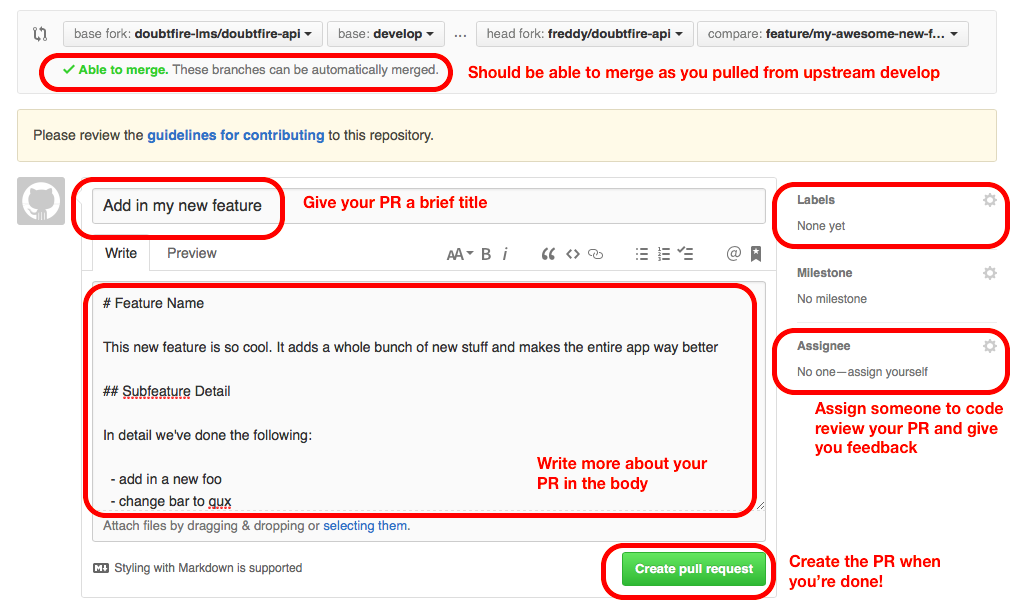
\includegraphics{43f3131730.png}
\caption{Feature Branches}
\end{figure}

We try to keep two main branches at all times:

\begin{itemize}
\tightlist
\item
  \texttt{master} for production
\item
  \texttt{develop} for current development, a branch off \texttt{master}
\end{itemize}

That way, we follow the workflow:

\begin{enumerate}
\def\labelenumi{\arabic{enumi}.}
\tightlist
\item
  branch off \texttt{develop}, giving your branch one of the prefixes
  defined below,
\item
  make your changes in that branch,
\item
  merge your branch back into \texttt{develop},
\item
  delete your branch to clean up
\end{enumerate}

In some cases, your branches may only consist of one or two commits.
This is still okay as you can submit a pull request for code review back
into \texttt{develop}.

You may want to branch again, e.g.:

\begin{verbatim}
* master
|\
| \
| |
| (b1) develop
| |\
| | (b2) feature/my-new-feature
| | |\
| | | (b3) test/unit-tests-for-new-feature
| | |/
| | (m1)
| |/
| (m2)
| |\
| | (b4) fix/broken-thing
| |/
| (m3)
| /|
|/ |
(m4)
|  |
|  |
*  *
\end{verbatim}

Here, we:

\begin{enumerate}
\def\labelenumi{\arabic{enumi}.}
\tightlist
\item
  branched off \texttt{master} to create our \texttt{develop} branch, at
  \textbf{\texttt{b1}}
\item
  branched off \texttt{develop} to create a new feature under the new
  branch \texttt{feature/my-new-feature}, at \textbf{\texttt{b2}}
\item
  branched off \texttt{feature/my-new-feature} to create some unit tests
  for that feature under \texttt{test/unit-tests-for-new-feature}, at
  \textbf{\texttt{b3}}
\item
  merged those unit tests back into \texttt{feature/my-new-feature}, at
  \textbf{\texttt{m1}}
\item
  merged the new feature back into \texttt{develop}, at
  \textbf{\texttt{m2}}
\item
  found a new bug in the feature later on, so branched off
  \texttt{develop} into \texttt{fix/broken-thing}, at
  \textbf{\texttt{b4}}
\item
  after we fixed our bug, we merged \texttt{fix/broken-thing} back into
  \texttt{develop}, at \textbf{\texttt{m3}}
\item
  decide we're ready to release, so merge \texttt{develop} into
  \texttt{master}, at \textbf{\texttt{m4}}
\end{enumerate}

Note that along the way \textbf{we're deleting branches after we don't
need them}. This helps us keep \emph{short-lived} branches that don't go
\emph{stale} after months of inactivity, and prevents us from forgetting
about open branches. The only branch we kept open was \texttt{develop},
which we can always branch off for new, un-released changes again.

Ideally, any changes that are merged into \texttt{master} have been
\textbf{code-reviewed} before they were merged into \texttt{develop}.
\textbf{You should always code review before merging back into
\texttt{develop}}. You can do this by performing a Pull Request, where
the reviewer can see the changes you want to merge in to
\texttt{develop}.

\hypertarget{getting-started-with-the-forking-workflow}{\subsection{Getting
started with the Forking
Workflow}\label{getting-started-with-the-forking-workflow}}

\subsubsection{1. Forking and Cloning the
repository}\label{forking-and-cloning-the-repository}

\paragraph{Fork the Repo}\label{fork-the-repo}

To get a copy of a Doubtfire repositories on your user account, you will
need to fork it \emph{for each repository}:

\begin{figure}[htbp]
\centering
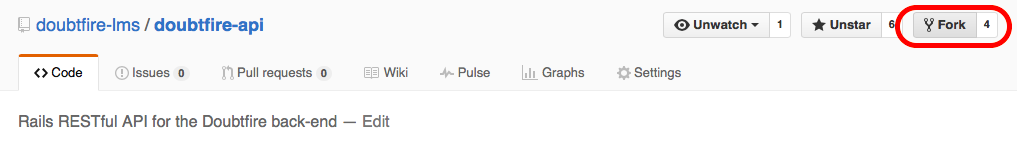
\includegraphics{68e50046d2.png}
\caption{Fork the repo}
\end{figure}

\paragraph{Clone the Fork}\label{clone-the-fork}

You can then clone the repositories you have forked to your machine. To
do so, navigate to your forked repositories and copy the clone URL:

\begin{figure}[htbp]
\centering
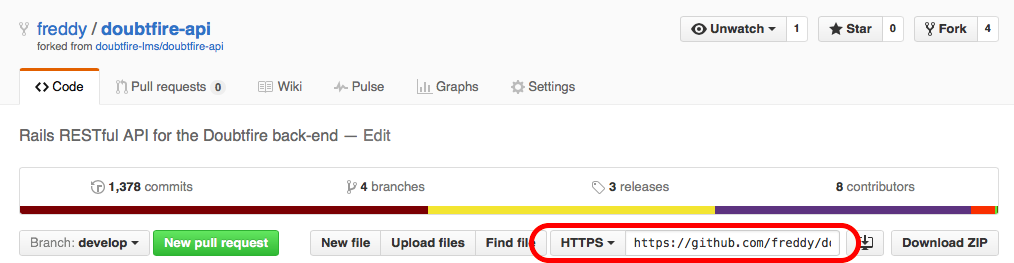
\includegraphics{a360d7c755.png}
\caption{Copy the clone URL}
\end{figure}

Navigate to your \texttt{projects} or \texttt{repo} folder, and make a
\texttt{doubtfire} folder. Then clone using the URLs you copied above:

\begin{verbatim}
$ cd ~/repos
$ mkdir doubtfire
$ cd doubtfire
$ git clone https://github.com/{username}/doubtfire-api.git
$ git clone https://github.com/{username}/doubtfire-web.git
\end{verbatim}

\paragraph{\texorpdfstring{Set up your upstream to
\texttt{doubtfire-lms}}{Set up your upstream to doubtfire-lms}}\label{set-up-your-upstream-to-doubtfire-lms}

By default, git tracks your remote forked repository (the repository you
cloned). This remote is called \texttt{origin}.

You will then need to set up a new remote to track to the
\texttt{doubfire-lms} owned repository. This will be useful when you
need to get the latest changes other developers have contributed to the
\texttt{doubtfire-lms} repo, but you do not yet have those changes in
your forked repo. Call this remote \texttt{upstream}:

\begin{verbatim}
$ cd ~/repos/doubtfire/doubtfire-api
$ git remote add upstream https://github.com/doubtfire-lms/doubtfire-api.git
$ cd ~/repos/doubtfire/doubtfire-web
$ git remote add upstream https://github.com/doubtfire-lms/doubtfire-web.git
\end{verbatim}

\paragraph{Ensure you have your author credentials set
up}\label{ensure-you-have-your-author-credentials-set-up}

You should ensure your git user config are set and set to the email
address you use with GitHub:

\begin{verbatim}
$ git config --global user.email "my-github-email@gmail.com"
$ git config --global user.name "Freddy Smith"
\end{verbatim}

\paragraph{Use a rebase pull}\label{use-a-rebase-pull}

We also want to avoid having merge commits whenever you pull from
\texttt{upstream}. It is useful to pull from upstream using the
\texttt{-\/-rebase} switch, as this avoids an unnecessary merge commit
when pulling if there are conflicts.

To fix this, always pull with \texttt{-\/-rebase} (unless otherwise
specified---see the \texttt{-\/-ff} switch needed in
\protect\hyperlink{3-prepare-for-a-pull-request}{Step 3}):

\begin{verbatim}
$ git pull upstream develop --rebase
\end{verbatim}

or alternatively, make a rebase pull as your default setting:

\begin{verbatim}
$ git config --global pull.rebase true
\end{verbatim}

\subsubsection{2. Writing your new
changes}\label{writing-your-new-changes}

As per the
\protect\hyperlink{about-the-doubtfire-branch-structure}{branching
structure}, you need to branch off of \texttt{develop} to a new branch
that will have your code changes in it. When branching, \textbf{be sure
you are using a \protect\hyperlink{branch-prefixes}{branch prefix}}:

\begin{verbatim}
$ cd ~/repos/doubtfire/doubtfire-api
$ git checkout -b feature/my-awesome-new-feature
\end{verbatim}

You can now begin making your changes. Commit along the way,
\textbf{being sure to conform to the
\protect\hyperlink{writing-commit-messages}{commit message guidelines}},
on this branch and push to your fork:

\begin{verbatim}
$ git status

On branch feature/my-awesome-new-feature
Your branch is up-to-date with 'origin/feature/my-awesome-new-feature'.
Changes not staged for commit:
  (use "git add <file>..." to update what will be committed)
  (use "git checkout -- <file>..." to discard changes in working directory)

  modified:   src/file-that-changed.js
  modified:   src/another-file-that-changed.js

$ git add src/file-that-changed.js src/another-file-that-changed.js
$ git commit

[feature/my-awesome-new-feature 7f35016] DOCS: Add new documentation about git
 2 files changed, 10 insertions(+), 15 deletions(-)

$ git push -u origin feature/my-awesome-new-feature
\end{verbatim}

Note you only need to add the \texttt{-u} flag on an initial commit for
a new branch.

\subsubsection{3. Prepare for a Pull
Request}\label{prepare-for-a-pull-request}

\textbf{Note, while it is advised you perform this step, it you can skip
it and move straight to the
\protect\hyperlink{4-submitting-a-pull-request-pr-to-the-upstream-repository}{Pull
Request step}. If the branch cannot be automatically merged, then you
should run through these steps.}

When you are done with your changes, you need to pull any changes from
\texttt{develop} from the \texttt{upstream} repository. This essentially
means ``get me anything that has changed on the \texttt{doubtfire-lms}
repository that I don't yet have''.

To do this, pull any changes (if any) from the \texttt{upstream}
repository's \texttt{develop} branch into your local \texttt{develop}
branch:

\begin{verbatim}
$ git checkout feature/my-awesome-new-feature
$ git pull --ff upstream develop
\end{verbatim}

If there are merge conflicts, you can resolve them now. Follow GitHub's
\href{https://help.github.com/articles/resolving-a-merge-conflict-from-the-command-line}{guide}
for resolving merge conflicts.

We can now update your \texttt{origin} repository's
\texttt{my-awesome-new-feature} on GitHub such that it will include the
changes from \texttt{upstream}:

\begin{verbatim}
$ git push origin feature/my-awesome-new-feature
\end{verbatim}

\subsubsection{4. Submitting a Pull Request (PR) to the upstream
repository}\label{submitting-a-pull-request-pr-to-the-upstream-repository}

Once you have pushed your changes to your fork, and have ensured nothing
has broken, you can then submit a pull request for code review to
Doubtfire.

To submit a pull request, go to the relevant Doubtfire LMS Repo and
click ``New Pull Request'':

\begin{figure}[htbp]
\centering
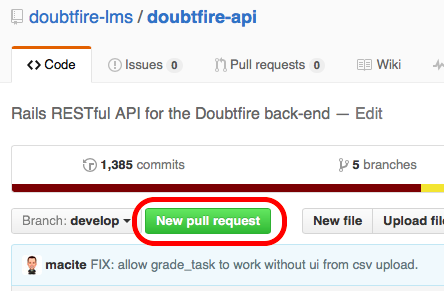
\includegraphics{77cd489a7f.png}
\caption{New PR}
\end{figure}

Ensure that the \textbf{Head Fork} is set to your forked repository and
on your feature branch. If you cannot see your repository, try clicking
the ``Compare across forks'' link.

\begin{figure}[htbp]
\centering
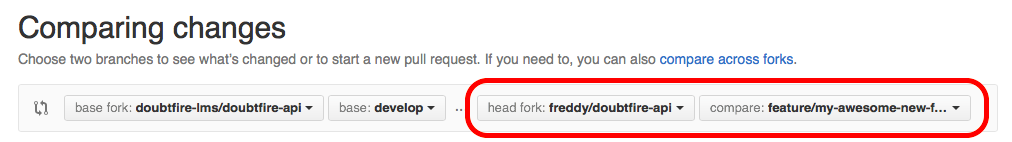
\includegraphics{22d554103e.png}
\caption{Compare forks}
\end{figure}

You can then begin writing the pull request. Be sure you are
\textbf{Able to Merge}, otherwise \textbf{try repeating an upstream pull
of develop into your feature branch, as per the
\protect\hyperlink{3-prepare-for-a-pull-request}{previous step}}.

\begin{figure}[htbp]
\centering
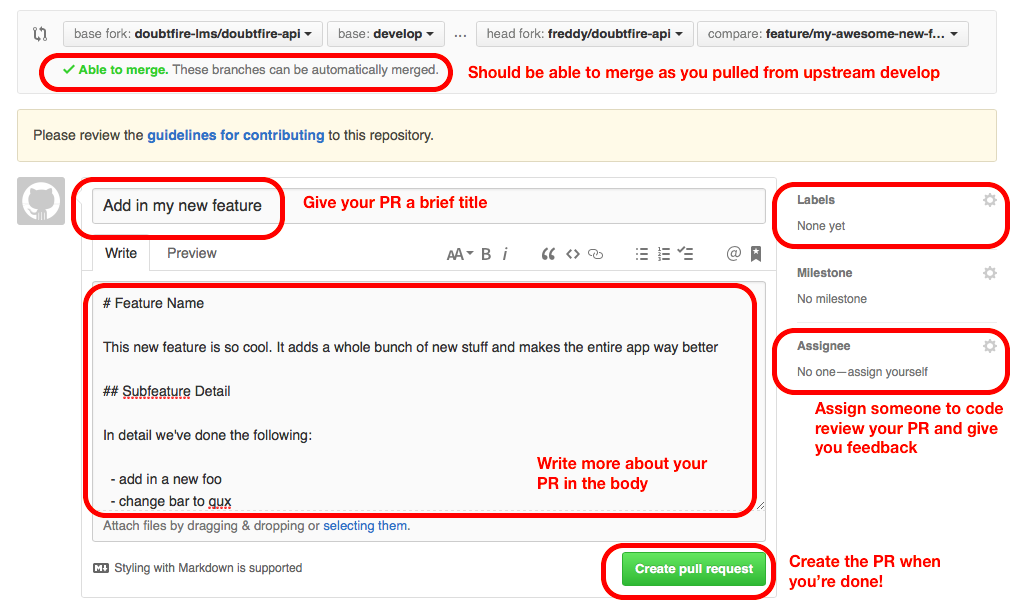
\includegraphics{8d3c8789a6.png}
\caption{Writing a Pull Request}
\end{figure}

With your PR body, be descriptive. GitHub may automatically add a commit
summary in the body. If fixing a problem, include a description of the
problem you're trying to fix and why this PR fixes it. When you are
done, assign a code reviewer and add a tag (if applicable) and create
the pull request!

If your code is ok, it will be merged into \texttt{develop}, (and
eventually \texttt{master}, meaning your code will go live - woohoo
:tada:)

If not, the reviewer will give you suggestions and feedback for you to
fix your code.

\textbf{STOP! Continue to the next step once your Pull Request is
approved and merged into the \texttt{doubtfire-lms}'s \texttt{develop}
branch.}

\subsubsection{5. Cleaning Up}\label{cleaning-up}

Once your pull request is approved, your code changes are finalised, and
merged you will want to delete your old feature branch so you don't get
lots of old branches on your repository.

Following from the example above, we would delete
\texttt{feature/my-awesome-new-feature} as it has been merged into
\texttt{develop}. We first delete the branch locally:

\begin{verbatim}
$ git branch -D feature/my-awesome-new-feature
\end{verbatim}

Then remove it from your fork on GitHub:

\begin{verbatim}
$ git push origin --delete feature/my-awesome-new-feature
\end{verbatim}

Then ensure you are git is no longer tracking the deleted branch from
\texttt{origin} by running a fetch prune:

\begin{verbatim}
$ git fetch --prune
\end{verbatim}

As your changes have been merged into \texttt{upstream}'s
\texttt{develop} branch, pull from \texttt{upstream} and you can grab
those changes into your local repository:

\begin{verbatim}
$ git checkout develop
$ git pull upstream develop
\end{verbatim}

Then push those changes up into your \texttt{origin}'s \texttt{develop}
so that it is synced with \texttt{upstream}'s \texttt{develop}:

\begin{verbatim}
$ git push origin upstream
\end{verbatim}

\hypertarget{workflow-summary}{\subsubsection{Workflow
Summary}\label{workflow-summary}}

\textbf{Step 1.} Set up for new feature branch:

\begin{Shaded}
\begin{Highlighting}[]
\NormalTok{$ }\KeywordTok{git} \NormalTok{checkout develop                    }\CommentTok{# make sure you are on develop}
\NormalTok{$ }\KeywordTok{git} \NormalTok{pull --rebase upstream develop      }\CommentTok{# sync your local develop with upstream's develop}
\NormalTok{$ }\KeywordTok{git} \NormalTok{checkout -b my-new-branch           }\CommentTok{# create your new feature branch}
\end{Highlighting}
\end{Shaded}

\noindent
\textbf{Step 2.} Make changes, and repeat until you are done:

\begin{Shaded}
\begin{Highlighting}[]
\NormalTok{$ }\KeywordTok{git} \NormalTok{add ... }\KeywordTok{;} \KeywordTok{git} \NormalTok{commit }\KeywordTok{;} \KeywordTok{git} \NormalTok{push     }\CommentTok{# make changes, commit, and push to origin}
\end{Highlighting}
\end{Shaded}

\noindent
\textbf{Step 3.} Submit a
\protect\hyperlink{4-submitting-a-pull-request-pr-to-the-upstream-repository}{pull
request}, and \textbf{if unable to merge}:

\begin{Shaded}
\begin{Highlighting}[]
\NormalTok{$ }\KeywordTok{git} \NormalTok{pull --ff upstream develop          }\CommentTok{# merge upstream's develop in your feature branch}
\NormalTok{$ }\KeywordTok{git} \NormalTok{add ... }\KeywordTok{;} \KeywordTok{git} \NormalTok{commit                }\CommentTok{# resolve merge conflicts and commit}
\NormalTok{$ }\KeywordTok{git} \NormalTok{push origin                         }\CommentTok{# push your merge conflict resolution to origin}
\end{Highlighting}
\end{Shaded}

\noindent
\textbf{Step 4.} Only when the pull request has been \textbf{approved
and merged}, clean up:

\begin{Shaded}
\begin{Highlighting}[]
\NormalTok{$ }\KeywordTok{git} \NormalTok{checkout develop                    }\CommentTok{# make sure you are back on develop}
\NormalTok{$ }\KeywordTok{git} \NormalTok{branch -D my-new-branch             }\CommentTok{# delete the feature branch locally}
\NormalTok{$ }\KeywordTok{git} \NormalTok{push --delete my-new-branch         }\CommentTok{# delete the feature branch on origin}
\NormalTok{$ }\KeywordTok{git} \NormalTok{fetch origin --prune                }\CommentTok{# make sure you no longer track the deleted branch}
\NormalTok{$ }\KeywordTok{git} \NormalTok{pull --rebase upstream develop      }\CommentTok{# pull the merged changes from develop}
\NormalTok{$ }\KeywordTok{git} \NormalTok{push origin develop                 }\CommentTok{# push to origin to sync origin with develop}
\end{Highlighting}
\end{Shaded}

\hypertarget{branch-prefixes}{\subsection{Branch
Prefixes}\label{branch-prefixes}}

When branching, try to prefix your branch with one of the following prefixes
shown in Table~\ref{tab:branches}.

\begin{sidewaystable}[]
\centering
\caption{Branch prefixes}
\label{tab:branches}
\vspace{1em}
\begin{tabular}{@{}lp{0.25\linewidth}l@{}}
\toprule
\textbf{Prefix} & \textbf{Description}                                                    & \textbf{Example}                         \\ \midrule
\texttt{feature/}        & New feature was added                                                   & \texttt{feature/add-learning-outcome-alignment  } \\
\texttt{fix/}            & A bug was fixed                                                         & \texttt{fix/crash-when-code-submission-finished } \\
\texttt{enhance/}        & Improvement to existing feature, but not visual enhancement (See \texttt{LOOKS}) & \texttt{enhance/allow-code-files-to-be-submitted} \\
\texttt{looks/}          & UI Refinement, but not functional change (See \texttt{ENHANCE})                  & \texttt{looks/rebrand-ui-for-version-2-marketing} \\
\texttt{quality/}        & Refactoring of existing code                                            & \texttt{quality/make-code-convention-consistent } \\
\texttt{doc/}            & Documentation-related changes                                           & \texttt{doc/add-new-api-documentation           } \\
\texttt{config/}         & Project configuration changes                                           & \texttt{config/add-framework-x-to-project       } \\
\texttt{speed/}          & Performance-related improvements                                        & \texttt{speed/new-algorithm-to-process-foo      } \\
\texttt{test/}           & Test addition or enhancement                                            & \texttt{test/unit-tests-for-new-feature-x       } \\ \bottomrule
\end{tabular}
\end{sidewaystable}

\hypertarget{writing-commit-messages}{\subsection{Writing Commit
Messages}\label{writing-commit-messages}}

Parts of this section have been adapted from Chris Beam's post,
\href{http://chris.beams.io/posts/git-commit/}{How to Write Good Commit
Messages}.

When writing commits, try to follow this guide as described in this subsection.

\hypertarget{prefix-your-commit-subject-line-with-a-tag}{\subsubsection{Prefix
your commit subject line with a
tag}\label{prefix-your-commit-subject-line-with-a-tag}}

Each one of your commit messages should be prefixed with one of the
following shown in Table~\ref{tab:tags}

\begin{sidewaystable}[]
\centering
\caption{Commit tagging guide}
\label{tab:tags}
\vspace{1em}
\begin{tabular}{@{}lp{0.25\linewidth}p{0.5\linewidth}@{}}
\toprule
Tag       & Description                                                             & Example                                                      \\ \midrule
\texttt{NEW}       & New feature was added                                                   & \textbf{NEW}: Add unit outcome alignment tab                          \\
\texttt{​FIX}      & A bug was fixed                                                         & \textbf{FIX}: Amend typo throwing error                               \\
\texttt{​​ENHANCE} & Improvement to existing feature, but not visual enhancement (See \texttt{LOOKS}) & \textbf{ENHANCE}: Calculate time between classes to show on timetable \\
\texttt{​LOOKS}    & UI Refinement, but not functional change (See \texttt{ENHANCE})                  & \textbf{LOOKS}: Make plagiarism tab consistent with other tabs        \\
\texttt{​QUALITY}  & Refactoring of existing code                                            & \textbf{QUALITY}: Make directives in consistent format with eachother \\
\texttt{​DOC}      & Documentation-related changes                                           & \textbf{DOC}: Write guide on writing commit messages                  \\
\texttt{CONFIG}    & Project configuration changes                                           & \textbf{CONFIG}: Add new scheme for UI automation testing             \\
\texttt{​SPEED}    & Performance-related improvements                                        & \textbf{SPEED}: Reduce time needed to batch process PDF submissions   \\
\texttt{TEST}      & Test addition or enhancement                                            & \textbf{TEST}: Add unit tests for tutorial administration             \\ \bottomrule
\end{tabular}
\end{sidewaystable}

\hypertarget{formatting-your-message}{\subsubsection{Formatting your
message}\label{formatting-your-message}}

Capitalise your commit messages and do not end the subject line with a
period

\begin{verbatim}
FIX: Change the behaviour of the logging system
\end{verbatim}

and not

\begin{verbatim}
fix: change the behaviour of the logging system.
\end{verbatim}

\hypertarget{use-the-imperative-mood-in-your-commit-subject-line}{\subsubsection{Use
the imperative mood in your commit subject
line}\label{use-the-imperative-mood-in-your-commit-subject-line}}

Write your commits in the imperative mood and not the indicative mood

\begin{itemize}
\tightlist
\item
  ``Fix a bug'' and \textbf{not} ``Fix\emph{ed} a bug''
\item
  ``Change the behaviour of Y'' and \textbf{not} ``\emph{Changed} the
  behaviour of Y''
\item
  ``Add new API methods'' and \textbf{not} ``Sweet new API methods''
\end{itemize}

A properly formed git commit subject line should always be able to
complete the following sentence:

\begin{quote}
If applied, this commit will \textbf{your subject line here}

If applied, this commit will \textbf{fix a bug}

If applied, this commit will \textbf{change the behaviour of Y}
\end{quote}

and not

\begin{quote}
If applied, this commit will \textbf{sweet new API methods}
\end{quote}

\hypertarget{subject-and-body-lines}{\subsubsection{Subject and body
lines}\label{subject-and-body-lines}}

Write a commit subject, and explain that commit on a new line (if need
be):

\begin{verbatim}
FIX: Derezz the master control program

MCP turned out to be evil and had become intent on world domination.
This commit throws Tron's disc into MCP (causing its deresolution)
and turns it back into a chess game.
\end{verbatim}

Keep the subject line (top line) concise; keep it \textbf{within 50
characters}.

Use the body (lines after the top line) to explain why and what and
\emph{not} how; keep it \textbf{within 72 characters}.

\paragraph{\texorpdfstring{But how can I write new lines if I'm using
\texttt{git\ commit\ -m\ "Message"}?}{But how can I write new lines if I'm using git commit -m "Message"?}}\label{but-how-can-i-write-new-lines-if-im-using-git-commit--m-message}

Don't use the \texttt{-m} switch. Use a text editor to write your commit
message instead.

If you are using the command line to write your commits, it is useful to
set your git editor to make writing a commit body easier. You can use
the following command to set your editor to \texttt{nano},
\texttt{emacs}, \texttt{vim}, \texttt{atom}.

\begin{verbatim}
$ git config --global core.editor nano
$ git config --global core.editor emacs
$ git config --global core.editor vim
$ git config --global core.editor "atom --wait"
\end{verbatim}

If you want to use Sublime Text as your editor, follow
\href{https://help.github.com/articles/associating-text-editors-with-git/\#using-sublime-text-as-your-editor}{this
guide}.

If you are not using the command line for git, you probably
\href{http://try.github.io}{should be}.

\end{document}
